\section*{\hypertarget{gameplay}{Gameplay}}
"You want quiet, you better take the next train."\\
\indent -- Lightning

\begin{center} 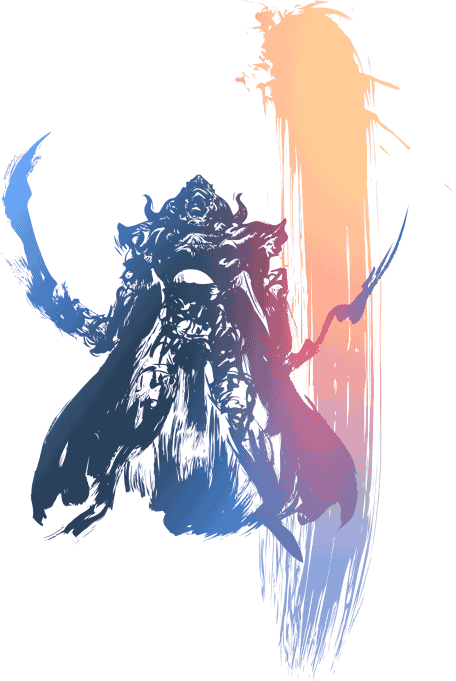
\includegraphics[width=\columnwidth]{./art/images/ff12.png} \end{center}

\addcontentsline{toc}{section}{Gameplay}

\subsubsection*{Introduction}
Final Fantasy is a series of roleplaying video games that has significantly shaped the genre since its first release in 1987.
Even though each Final Fantasy title features its unique story, setting and characters, they still feel very much as part of the same series.
This is not only due to many recurring elements that they have in common, but also because the stories focus on a group of heroes who face a great conflict.
\mbox{\textbf{Omega Fantasy}} is a tabletop game system that helps you and your friends to create and play in a Final Fantasy adventure of your own.

\vfill

\subsubsection*{Getting Started}
To play Omega Fantasy, you only need dice, paper, pens, this book and at least one more friend, but a group size of 4 to 6 is recommend.
Choose one person to become the \mbox{\textbf{Game Master}}, who creates the fantasy world and narrates the adventure.
Everyone else is a \textbf{Player}, who takes the role of one of the protagonists.
You do not need any prior knowledge of Final Fantasy or roleplaying, everything necessary is explained in the following.

\pagebreak

\subsubsection*{Players}
Players create and roleplay as \textbf{characters} who are the protagonists of the story.
They take the role of their characters and play the game from their perspective.  
These adventurers travel together as a \textbf{party}, who explore the world, interact with people and fight against enemies. 
Usually, the party is confronted with a \textbf{central conflict} by the game master, as the general goal of their adventure.
This book includes various rules and options that help you to create and develop your character.  

\subsubsection*{Game Master}
The Game Master (shortened \textbf{GM}), creates the world the adventure takes place in by using the content and guidelines in this book. 
During the game, he describes the environment to the party and how it reacts to their actions. 
The GM takes the role of all non-player characters to narrate conversations and combat. 
The rules in this book help the GM determine the outcome of some actions, though often he needs to make his own rulings.

\subsubsection*{Dice}
Dice rolls are used in various situations to help decide the outcome uncertain actions.
However, depending on its context, the exact nature of such a roll may differ. 
The only dice used in this game are standard six-sided ones and we often use \textbf{d} shorthand to refer to such a die.
Furthermore, we use for example "4d" to describe a roll of 4 dice, where the result is the sum of all rolled dice.

\vspace{1cm}

\example{Roleplaying}
{
	\begin{description}[leftmargin=*]
	\item[Hironobu (Game Master):]
	You enter the Thunder Plains, which is a vast wasteland covered by thick fog and dark clouds.
	The locals have erected towers, that act as lightning rods, but you can see that bolts often strike the ground in the open field.
	\item[Yoshinori (playing as Wakka):] We head north, not too near and not too far from the towers, ya?
	\item[Nobuo (playing as Rikku):] I wanna go home! I hate lightning! I hate thunder!
	\item[Tetsuya (playing as Auron):] This storm never stops. Better to cross quickly.
	\item[Hironobu (Game Master):] You can also see a small building nearby, that looks like an inn.
	\item[Nobuo (playing as Rikku):] Let’s go rest over there! Please? I'm too young to die!
	\item[Tetsuya (playing as Auron):] Fine, we rest. She is worse than the storm.
	\end{description}
}

\pagebreak
